% 3.绪论.tex 绪论（大气排版版）
\chapter{绪论}

% ===== 局部排版优化（仅影响本章，使版面更舒展）=====
\setlength{\parskip}{0.8ex plus 0.3ex minus 0.2ex}   % 段落间距增加
\setlist{
    leftmargin=2.5em,          % 列表左缩进增大
    itemsep=0.6em,             % 条目垂直间距
    parsep=0.3em,              % 条目内段落间距
    topsep=0.8em,              % 列表与上下文间距
    partopsep=0.3em
}
\renewcommand{\arraystretch}{1.5}      % 表格行高增加
\setlength{\tabcolsep}{10pt}           % 表格列间距增加
\addtolength{\abovedisplayskip}{2pt}   % 公式前间距微增
\addtolength{\belowdisplayskip}{2pt}   % 公式后间距微增
% ========================================

\bigskip  % 章节标题后额外留白

\section{自动控制理论的研究对象与任务}
自动控制理论是研究自动控制系统组成、分析与设计的工程学科，核心任务：通过控制方案设计，使被控对象的被控物理量（位移、转速、温度、电压等）严格按照预设参考规律变化。

\subsection{控制系统核心基本名词（必考名词解释）}
\begin{itemize}
    \item \textbf{被控对象}：待控制的设备/生产过程，典型实例：电机、温控箱体、机械弹簧阻尼系统、RLC电路；
    \item \textbf{输入量（给定信号/参考输入）}：系统参考指令，是输出量期望跟随的目标，记作$r(t)$；
    \item \textbf{输出量（被控量/系统输出）}：被控对象被调节的物理量，系统实际输出，记作$y(t)$；
    \item \textbf{干扰量（扰动）}：破坏输出量跟随给定、不受人为控制的外加扰动信号，记作$f(t)$；
    \item \textbf{反馈信号}：测量元件采集实际输出$y(t)$后得到的回馈信号，用于和输入做差值运算；
    \item \textbf{偏差信号}：输入与反馈信号的差值 $\varepsilon(t)=r(t)-b(t)$，是控制器的驱动输入；
    \item \textbf{控制器}：依据偏差信号生成控制量的核心运算单元；
    \item \textbf{执行元件}：接收控制量，直接驱动被控对象改变被控量。
\end{itemize}

\section{控制系统分类（考试选择/填空/简答题考点）}
\subsection{1. 按信号连接方式：开环/闭环控制系统}
\begin{enumerate}
    \item \textbf{开环控制系统}：无反馈通路，输出不影响输入；结构简单、成本低、调试简便，但抗干扰能力差、控制精度低，元件参数漂移对输出影响大；
    \item \textbf{闭环（反馈）控制系统}：引入输出反馈构成闭合回路，利用偏差消除误差；抗干扰强、控制精度高、元件参数变化影响小，是本课程研究主体；缺点为结构复杂、造价高、调试难度大。
\end{enumerate}

\begin{table}[htbp]
\centering
\caption{开环、闭环控制系统优缺点对比}
\begin{tabular}{@{}lcc@{}}
\toprule
& 开环控制系统 & 闭环控制系统 \\
\midrule
优点 & 结构简单、造价低、调试简易 & 控制精度高、抗干扰强、元件漂移影响小 \\
缺点 & 精度差、无抗扰能力、参数波动影响大 & 结构复杂、成本高、调试繁琐 \\
\bottomrule
\end{tabular}
\end{table}

\paragraph{闭环系统五大组成器件（简答考点）}
\begin{itemize}
    \item 比较元件：完成输入与反馈的求差运算，生成偏差信号；
    \item 放大元件：放大微弱偏差信号，提供驱动功率；
    \item 校正元件：串联/并联接入，用于改善系统动态、稳态性能；
    \item 执行元件：接收控制信号，直接驱动被控对象改变输出；
    \item 测量元件：实时采集实际输出，生成反馈信号。
\end{itemize}

\subsection{2. 按系统微分方程特性分类（核心分类，期末高频）}
依据微分方程系数与是否含非线性项，分为四类：
\begin{enumerate}
    \item \textbf{线性定常系统（LTI）}：微分方程全部为一次线性项、各项系数均为常数；满足叠加原理，是本课程重点研究对象；
    \[
    m\ddot{y}(t)+f\dot{y}(t)+ky(t)=F(t)
    \]
    \item \textbf{线性时变系统（LTV）}：方程为线性，但至少一个系数随时间$t$变化：$\dot{y}(t)+a(t)y(t)=bu(t)$；
    \item \textbf{非线性定常系统（NLTI）}：方程包含$\sin y$、$y^2$等非线性项，系数为常数；\textbf{不满足叠加原理}；
    \item \textbf{非线性时变系统（NLTV）}：同时含有非线性项+时变系数，工程最难分析。
\end{enumerate}

\subsection{3. 其他常见分类（识记即可）}
\begin{itemize}
    \item 按输入输出维度：单输入单输出（SISO，经典控制研究范畴）、多输入多输出（MIMO，现代控制范畴）；
    \item 按时间信号形式：连续时间系统、离散采样系统（Z变换章节内容）；
    \item 按输入规律：恒值控制系统、随动（伺服）控制系统；
    \item 按随机属性：确定性系统、随机不确定系统。
\end{itemize}

\section{典型物理系统微分方程（建模必考，机械+电气）}
\subsection{机械平移系统（质量-弹簧-阻尼模型）}
$m$：质量，$f$：粘性阻尼系数，$k$：弹簧刚度；$F(t)$为外加输入力，$y(t)$为质量块位移输出：
\[
m \frac{d^2 y(t)}{dt^2} + f \frac{d y(t)}{dt} + k y(t) = F(t)
\]

\subsection{RLC串联电气系统}
$R$电阻、$L$电感、$C$电容；$u_i(t)$输入电压，$u_o(t)$电容两端输出电压：
\[
LC \frac{d^2 u_o(t)}{dt^2} + RC \frac{du_o(t)}{dt} + u_o(t) = u_i(t)
\]

\section{控制系统四大性能指标（全书总纲领，简答必背）}
评判控制系统性能的四项核心指标：稳定性、快速性、准确性、平稳性。
\begin{enumerate}
    \item \textbf{稳定性}：系统固有属性，仅由系统结构参数决定，与输入信号无关；扰动消失后输出可收敛回稳态（或对于有界输入，输出有界），是系统正常工作的先决条件；不稳定系统会发散振荡，无实用工程价值；
    \item \textbf{快速性}：表征系统暂态动态特性，衡量被控量趋近期望值的响应快慢；用时域上升时间、调节时间量化；
    \item \textbf{准确性}：表征系统稳态静态特性，动态过程结束后，实际输出与期望输入的差值，用稳态误差定量描述；
    \item \textbf{平稳性}：表征系统暂态动态特性，描述动态过程中超调量与振荡幅度，振荡越小平稳性越好。
\end{enumerate}

\section{典型测试输入信号（识记考点）}
\begin{table}[htbp]
\centering
\caption{典型测试信号波形}
\begin{tabular}{ccc}
单位阶跃 $1(t)$ & 单位斜坡 $t\cdot1(t)$ & 单位脉冲 $\delta(t)$ \\[5pt]
\begin{tikzpicture}[scale=0.7, baseline=(current bounding box.center)]
\draw[->] (-0.5,0) -- (2.2,0) node[right] {$t$};
\draw[->] (0,-0.2) -- (0,1.2) node[above] {};
\draw (0,0) -- (0,1);
\draw[thick] (0,1) -- (2,1);
\fill (0,0) circle (1.2pt);
\end{tikzpicture} &
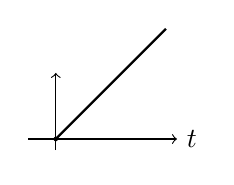
\begin{tikzpicture}[scale=0.7, baseline=(current bounding box.center)]
\draw[->] (-0.5,0) -- (2.2,0) node[right] {$t$};
\draw[->] (0,-0.2) -- (0,1.2) node[above] {};
\draw[thick] (0,0) -- (2,2);
\fill (0,0) circle (1.2pt);
\end{tikzpicture} &
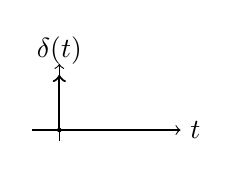
\begin{tikzpicture}[scale=0.7, baseline=(current bounding box.center)]
\draw[->] (-0.5,0) -- (2.2,0) node[right] {$t$};
\draw[->] (0,-0.2) -- (0,1.2) node[above] {};
\draw[->, thick] (0,0) -- (0,1) node[above] {$\delta(t)$};
\fill (0,0) circle (1.2pt);
\end{tikzpicture} \\[15pt]
\multicolumn{3}{c}{单位正弦 $\sin\omega t$} \\[5pt]
\multicolumn{3}{c}{
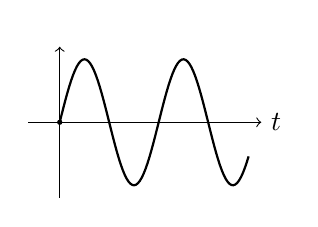
\begin{tikzpicture}[scale=0.8, baseline=(current bounding box.center)]
\draw[->] (-0.5,0) -- (3.2,0) node[right] {$t$};
\draw[->] (0,-1.2) -- (0,1.2) node[above] {};
\draw[domain=0:3, thick, samples=100] plot(\x,{sin(4*\x r)});
\fill (0,0) circle (1.2pt);
\end{tikzpicture}
} \\
\end{tabular}
\end{table}

\begin{itemize}
    \item \textbf{单位阶跃信号}：瞬时阶跃跳变输入，用于考核系统稳态误差与动态响应；
    \item \textbf{单位斜坡信号}：随时间线性增长输入，考核匀速跟踪误差；
    \item \textbf{单位脉冲信号}：单位瞬时冲击信号，用于求解系统单位脉冲响应；
    \item \textbf{单位正弦信号}：周期性交变输入，是频域分析法的基准激励。
\end{itemize}

\section{课程内容导航（全书框架识记）}
本课程整体分为\textbf{系统建模、系统分析、系统综合}三大板块：
\begin{enumerate}
    \item \textbf{控制系统数学建模}：包含微分方程、传递函数、结构图、信号流图四种建模方法；
    \item \textbf{控制系统性能分析}：分为时域分析法、根轨迹分析法、频域分析法；
    \item \textbf{控制系统综合校正（设计）}，细分三条设计路线：
    \begin{itemize}
        \item 基于传递函数+根轨迹法：\textbf{根轨迹校正}；
        \item 基于频率响应法：\textbf{频率域校正}；
        \item 非线性控制系统：采用\textbf{相平面法}分析与校正。
    \end{itemize}
\end{enumerate}

% ===== 恢复全局默认间距（避免影响后续章节）=====
\setlength{\parskip}{0pt plus 1pt}
\setlist{leftmargin=2em, itemsep=0.2em, parsep=0pt}
\renewcommand{\arraystretch}{1}
\setlength{\tabcolsep}{6pt}
% ============================================